\section{\texorpdfstring{
\includegraphics[width=150pt]{redux.png}}{Redux}}

\begin{frame}

  \frametitle{Redux}
  Redux is a predictable state container for JavaScript apps.

	\textbf{Three Principles}

	Single source of truth

	State is read-only

	Changes are made with pure functions 

\end{frame}

\begin{frame}

  \frametitle{Architecture of a redux app}
	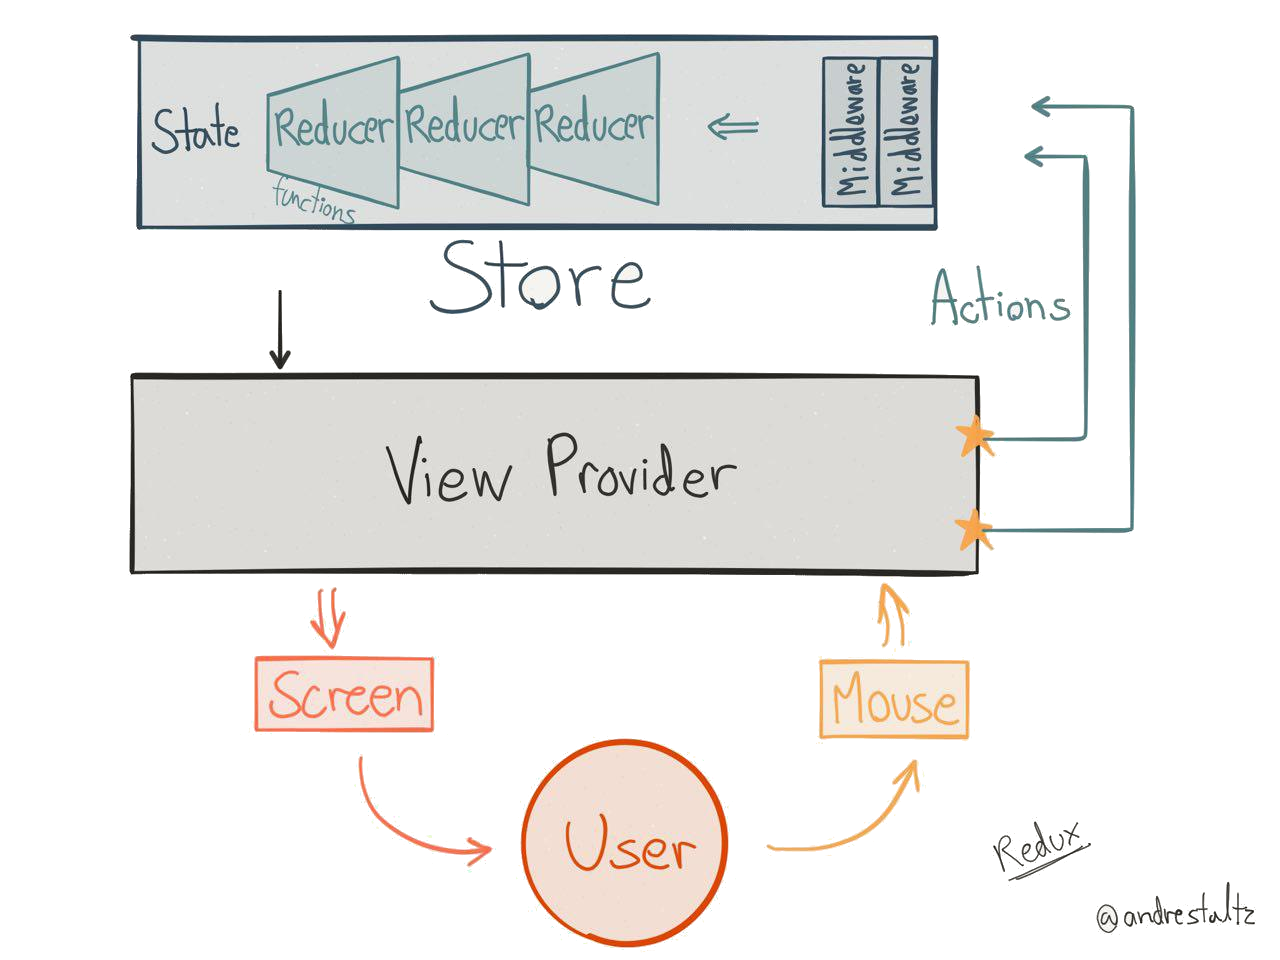
\includegraphics[width=\textwidth]{redux-unidir-ui-arch.png}

\end{frame}

\begin{frame}[fragile]
	\frametitle{Actions}
  Payloads of information that send data from your application to your store. They are the only source of information for the store. You send them to the store using \textit{store.dispatch()}.

	\begin{minted}[fontsize=\tiny]{javascript}
  const action = { type: 'TOGGLE_TODO', index: 6 }  // 'type' is the only thing required
	\end{minted}

  \textbf{Action creators} are functions that return actions

	\begin{minted}[fontsize=\tiny]{javascript}
  function addTodo (text) {
    returns { type: 'ADD_TODO', text }
  }

  store.dispatch(addTodo('Pray to Yisus'))

  const boundAddTodo = text => store.dispatch(addTodo(text))
  boundAddTodo('Pray to Yisus')
	\end{minted}

\end{frame}

\begin{frame}[fragile]
  \frametitle{Reducers}
  Specify how the application's state changes in response to actions.

  \begin{multicols}{2}
  \footnotesize State
	\begin{minted}[fontsize=\tiny]{javascript}
  {
    visibilityFilter: 'SHOW_ALL',
    todos: [
      {
        text: 'Consider using Redux',
        completed: true,
      },
      {
        text: 'Keep all state in a single tree',
        completed: false
      }
    ]
  }
  \end{minted}

  \columnbreak

  \footnotesize Action
	\begin{minted}[fontsize=\tiny]{javascript}
{
  type: 'SET_VISIBILITY_FILTER',
  filter: 'SHOW_FINISHED'
}
  \end{minted}

  \end{multicols}
\end{frame}

\begin{frame}[fragile]
  \frametitle{Reducers}

  \small The reducer is a pure function \textit{(previousState, action) => newState}

  \begin{minted}[fontsize=\tiny]{javascript}
function todoApp (state = initialState, action) {  // initializes the state
  switch (action.type) {  // looks the type of the action
    case SET_VISIBILITY_FILTER:
      return Object.assign({}, state, {  // returns the new state object
        visibilityFilter: action.filter  // with the changed visibility filter
      })
    case ADD_TODO:
      return Object.assign({}, state, {
        todos: [
          ...state.todos,
          {
            text: action.text,
            completed: false
          }
        ]
      })    
    default:
      return state
  }
}
  \end{minted}
\end{frame}

\begin{frame}[fragile]
  \frametitle{Reducers composition}
  \begin{multicols}{2}
    \scriptsize One reducer for each part of the tree
    \begin{minted}[fontsize=\tiny]{javascript}
function visibilityFilter(
    state = SHOW_ALL, action
  ) {
  switch (action.type) {
    case SET_VISIBILITY_FILTER:
      return action.filter
    default:
      return state
  }
}

function todos (state = [], action) {
  switch (action.type) {
    case ADD_TODO:
      return [
        ...state,
        {
          text: action.text,
          completed: false
        }
      ]
    default:
      return state
  }
}
    \end{minted}

  \columnbreak

    \scriptsize State 
    \begin{minted}[fontsize=\ssmall]{javascript}
{ visibilityFilter: 'SHOW_ALL',
  todos: [
    { text: 'Consider using Redux',
      completed: true, },
    { text: 'Keep all state in a single tree',
      completed: false } ] }

    \end{minted}

    \scriptsize All the reducers are combined in one
    \begin{minted}[fontsize=\tiny]{javascript}
function todoApp (state = {}, action) {
  return {
    visibilityFilter: visibilityFilter(
      state.visibilityFilter, action),
    todos: todos(state.todos, action)
  }
}

// Redux let's us do it with combineReducers

import { combineReducers } from 'redux'

const todoApp = combineReducers({
  visibilityFilter,
  todos
})
    \end{minted}

  \end{multicols}
\end{frame}

\begin{frame}[fragile]
  \frametitle{Store API}
  \begin{multicols}{2}
    \footnotesize Implementation
    \begin{minted}[fontsize=\tiny]{javascript}
const createStore = reducer => {
  let state
  let listener = []

  const getState = () => state

  const dispatch = action => {
    state = reducer(state, action)
    listeners.forEach(
      listener => listener()
    )
  }

  const subscribe = listener => {
    listeners.push(listener)
    return () => {
      listeners = listeners.filter(
        l => l !== listener
      )
    }
  }
}
    \end{minted}

  \columnbreak

    \footnotesize Usage
    \begin{minted}[fontsize=\tiny]{javascript}
import { createStore } from 'redux'
import todoApp from './reducers'
let store = createStore(todoApp)

// Every time the state changes, log it
// Note that subscribe() returns a function 
// for unregistering the listener
let unsubscribe = store.subscribe(() =>
  console.log(store.getState())
)

// Dispatch some actions
store.dispatch(addTodo('Learn about actions'))
store.dispatch(addTodo('Learn about reducers'))
store.dispatch(addTodo('Learn about store'))
store.dispatch(
  setVisibilityFilter(
    VisibilityFilters.SHOW_COMPLETED
  )
)

// Stop listening to state updates
unsubscribe()
    \end{minted}
  \end{multicols}
\end{frame}

\begin{frame}[fragile]
  \frametitle{React integration}
  \begin{minted}[fontsize=\tiny]{javascript}
import { setFilter } from 'actions'

export default class ChangeFilter extends Component {  // Usage <ChangeFilter store=store />
  componentDidMount () {
    this.unsubscribe =   // The return value of subscribe is an unsubscribe method
      this.props.store.subscribe(  // Subscribe to store changes 
        () => this.forceUpdate())  // Update the component when something changes
  }

  componentWillUnmount () {
    this.unsubscribe()  // Unsubscribe from store change notifications
  }

  render () {
    const store = this.props.store
    const state = store.getState()  // Read the state of the store
    return ( 
      <div>
        Current filter {state.visibilityFilter}  // Read a value from the store
        <Button onClick={() => store.dispatch(  // Dispatch and action to update the store
          setFilter('SHOW_ALL')  // Action creator
        )} >
          SHOW ALL
        </Button>
      </div> 
    ) 
  } 
}
  \end{minted}
\end{frame}

\begin{frame}[fragile]
  \frametitle{React integration}
  \begin{multicols*}{2}
  \footnotesize With \textbf{react-redux}
  \begin{minted}[fontsize=\tiny]{javascript}
import { setFilter } from 'actions'
import { connect } from 'react-redux'

const ChangeFilter = props => {
  return (<div>
    Current filter {prop.visibilityFilter}
    <Button onClick={() => props.dispatchSetFilter('SHOW_ALL')} >
      SHOW ALL
    </Button>
  </div> ) } }
}

function mapStateToProp (state, props) {
  return {  // This will be passed as props
    visibilityFilter = state.visibilityFilter  
  }
}

function mapStateToDispatch (dispatch, props) {
  return {  // This will be passed as props
    dispatchSetFilter: filter => dispatch(setFilter(filter))
  }
}

export default connect (mapStateToProps, mapDispatchToProps)(ChangeFilter)
  \end{minted}
  \columnbreak
  \begin{minted}[fontsize=\ssmall]{javascript}
// main.jsx where App includes our ChangeFilter
render( 
  <Provider store={store}> <App /> </Provider>,
  document.getElementById('root')
)
  \end{minted}
  \end{multicols*}
\end{frame}
